\section{Linear Algebra Strategy}
\label{strategy}
\indent
\subsection{Towards a linear algebra semantics for SQL}

Inspired by point-free relational data processing, an alternative roadmap for parallel online analytical processing (OLAP) can be achieved based on encoding data in matrix format and relying thereupon solely on LA operations\cite{macedo2011middle}. 

\subsubsection{Encoding data in matrix format}

As example of raw data consider the displayed table \ref{table:example_table} where each row records the order key, quantity, return flag, line status and ship date from an given TPC-H benchmark lineitem table. In order to facilitate data association the column number in the corresponding lineitem table was included above each data column.
% !TEX encoding = UTF-8 Unicode

\begin{table}[H]


\caption{ Collection of raw data (adapted from TPC-H benchmark lineitem table). }
\label{table:example_table}
\scriptsize
\centering
\begin{tabular}{ |  L{1.5cm} |  L{1.5cm}  |  L{1.5cm}  |  L{1.5cm}  |  L{1.5cm} |   } 
\hline
\#1	&	\#5	&	\#9	&	\#10	&	\#11	  \\ 
l\_orderkey	&	l\_quantity	&	l\_returnflag	&	l\_linestatus	&	 l\_shipdate 	  \\ \hline
\hline
1	&	17	&	N	&	O	&	1996-03-13	  \\ \hline
1	&	36	&	N	&	O	&	1996-04-12	  \\ \hline
1	&	8	&	N	&	O	&	1996-01-29	  \\ \hline
1	&	28	&	N	&	O	&	1996-04-21	  \\ \hline
1	&	24	&	N	&	O	&	1996-03-30	  \\ \hline
1	&	32	&	N	&	O	&	1996-01-30	  \\ \hline
2	&	38	&	N	&	O	&	1997-01-28	  \\ \hline
3	&	45	&	R	&	F	&	1994-02-02	  \\ \hline
3	&	49	&	R	&	F	&	1993-11-09	  \\ \hline
3	&	27	&	A	&	F	&	1994-01-16	  \\ \hline
\end{tabular}
\end{table}


To obtain useful information from raw data, which in OLAP systems escalated to Terabytes of information, we need to summarise the data by selecting attributes of interest and exhibiting their inter-relationships.\par 
Consider the following simplified TPC-H query 1: "How many items were sold per return flag and line status?". For this particular question, the necessary attributes to answer the query are present on table lineitem, being \textbf{return flag}, \textbf{line status}, and \textbf{quantity}. In relational algebra that question could be easily expressed by the following SQL code, which would produce the result presented on table \ref{table:results_simple_query_1}.

\lstinputlisting[caption=SQL code for the simplified TPC-H query 1, label=simple_query_1]{sql/simple_query_1.sql} %input de um ficheiro


% !TEX encoding = UTF-8 Unicode
\begin{table}[H]
\caption{Simplified query-1 relational algebra result from the collection of raw data (adapted from TPC-H benchmark lineitem table). }
\label{table:results_simple_query_1}
\scriptsize
\centering
\begin{tabular}{ |  L{1.5cm} |  L{1.5cm}  |  L{1.5cm}  |    } 
\hline
\#9	&	\#10		 & \#5	  \\ 
l\_returnflag	&	l\_linestatus	&	 l\_quantity 	  \\ \hline
\hline
N	&	O	&	183	  \\ \hline
R	&	F	&	94	  \\ \hline
A	&	F	&	27	  \\ \hline
\end{tabular}

\end{table}


Aggregations like the ones presented on this query occur in all TPC-H queries, hence performance of group-by and aggregation deserves a special attention.
This issue will be addressed in later sections of the report.\par 
To express OLAP queries in therms of LA, the key lies in expressing operations in the form of matrix algebra expressions. 
This particular example, requires three matrices, one for each attribute, with each matrix being correlated to relational algebra as the row storage of columns \#5, \#9, and \#10.

However, to do so, we need to find a two-way association between the presented string on the rows \#9 and \#10 and an unique integer identifier. 

Our proposed solution encodes strings recurring to Gnome \textbf{Gquarks} - a two-way association between a non-zero unsigned int and a char * - based on a thread safe hashtable. \par 

By order of appearance, each unique string will be associated to an unique unsigned integer. Repeated strings will be associated to the prior corresponding unsigned integer. The resulting unsigned integer value range will start in the number 1. 

The value 0 in GQuarks is associated to NULL. 
Since in the proposed solution, row and column numbers will respect C-style arrays notation, both column and row numbering will start at 0. 

The GQuark unsigned integer value decremented by 1  will represent the row position on the matrix, and the register number, starting at 0, will represent the column position on the matrix. \par 
We can now verify that at most one non-zero cell can be found in each column of the matrix, to maintain the two-way association between a register and its corresponding string (the matrix is "functional"). There is also the possibility of direct associating an register number with a value, wether integer or floating point. The referred matrices will be diagonal matrices, in which the element value is directly associated with the register.\par 
Two types of matrices have now been presented:
\label{definition_matrices}
\begin{enumerate}
\item Projection matrices - which recur to Gnome Gquarks, in which the Gquark decremented by 1, represents the row position of the matrix, and the register number, starting at 0,  represents the column position on the matrix.
\item Measure matrices -  direct associating a register number with a value, wether integer or floating point,  where the element value is directly associated with the register number, and consequently the column and row position.
\end{enumerate}
 
We can now build the necessary matrices for the given examples, as shown in figures  \ref{fig:example_matrix_5} to \ref{fig:example_matrix_10}. The two-way association between char* and unsigned integer is also presented in table \ref{table:association_quarks_row}, to aid the example comprehension. 

% !TEX encoding = UTF-8 Unicode
\begin{table}[H]
\caption{Two-Way association between GQuarks and Row Number, for rows \#9 and \#10 presented in the collection of raw data (adapted from TPC-H benchmark lineitem table). }
\label{table:association_quarks_row}
\scriptsize
\centering
\begin{tabular}{ |  L{1.5cm} |  L{1.5cm}  |  L{1.5cm}  |    } 
\hline
String	&	GQuark	&	Row \#	  \\ \hline
\hline
N	&	1	&	0	  \\ \hline
R	&	2	&	1	  \\ \hline
A	&	3	&	2	  \\ \hline
O	&	4	&	3	  \\ \hline
F	&	5	&	4	  \\ \hline
\end{tabular}

\end{table}


  \begin{figure}[H]
    \centering
    \caption{Dense measure matrix produced from the collection of raw data (adapted from TPC-H benchmark lineitem table), from column \#5 (quantity column).}
\[
\begin{blockarray}{ccccccccccc}
	&	c0	&	c1	&	c2	&	c3	&	c4	&	c5	&	c6	&	c7	&	c8	&	c9	\\
\begin{block}{c(cccccccccc)}
r0	&	17	&	0	&	0	&	0	&	0	&	0	&	0	&	0	&	0	&	0	\\
r1	&	0	&	36	&	0	&	0	&	0	&	0	&	0	&	0	&	0	&	0	\\
r2	&	0	&	0	&	8	&	0	&	0	&	0	&	0	&	0	&	0	&	0	\\
r3	&	0	&	0	&	0	&	28	&	0	&	0	&	0	&	0	&	0	&	0	\\
r4	&	0	&	0	&	0	&	0	&	24	&	0	&	0	&	0	&	0	&	0	\\
r5	&	0	&	0	&	0	&	0	&	0	&	32	&	0	&	0	&	0	&	0	\\
r6	&	0	&	0	&	0	&	0	&	0	&	0	&	38	&	0	&	0	&	0	\\
r7	&	0	&	0	&	0	&	0	&	0	&	0	&	0	&	45	&	0	&	0	\\
r8	&	0	&	0	&	0	&	0	&	0	&	0	&	0	&	0	&	49	&	0	\\
r9	&	0	&	0	&	0	&	0	&	0	&	0	&	0	&	0	&	0	&	27	\\
\end{block}
\end{blockarray}
 \]
    \label{fig:example_matrix_5}
    \end{figure}
        
\begin{figure}[H]
\centering
\caption{Dense projection matrix produced from the collection of raw data (adapted from TPC-H benchmark lineitem table), from column \#9 (return flag column) with 2-way association achieved recurring to GQuarks.}
\[
\begin{blockarray}{ccccccccccc}
	&	c0	&	c1	&	c2	&	c3	&	c4	&	c5	&	c6	&	c7	&	c8	&	c9	\\
\begin{block}{c(cccccccccc)}
r0	&	1	&	1	&	1	&	1	&	1	&	1	&	1	&	0	&	0	&	0	\\
r1	&	0	&	0	&	0	&	0	&	0	&	0	&	0	&	1	&	1	&	0	\\
r2	&	0	&	0	&	0	&	0	&	0	&	0	&	0	&	0	&	0	&	1	\\
\end{block}
\end{blockarray}
\]
    \label{fig:example_matrix_9}
\end{figure}

\begin{figure}[H]
\centering
\caption{Dense projection matrix produced from the collection of raw data (adapted from TPC-H benchmark lineitem table), from column \#10 (line status column) with 2-way association achieved recurring to GQuarks.}
\[
\begin{blockarray}{ccccccccccc}
	&	c0	&	c1	&	c2	&	c3	&	c4	&	c5	&	c6	&	c7	&	c8	&	c9	\\
\begin{block}{c(cccccccccc)}
r0	&	0	&	0	&	0	&	0	&	0	&	0	&	0	&	0	&	0	&	0	\\
r1	&	0	&	0	&	0	&	0	&	0	&	0	&	0	&	0	&	0	&	0	\\
r2	&	0	&	0	&	0	&	0	&	0	&	0	&	0	&	0	&	0	&	0	\\
r3	&	1	&	1	&	1	&	1	&	1	&	1	&	1	&	0	&	0	&	0	\\
r4	&	0	&	0	&	0	&	0	&	0	&	0	&	0	&	1	&	1	&	1	\\
\end{block}
\end{blockarray}
\]
\label{fig:example_matrix_10}
\end{figure}
    
    \subsection{Projection Operation}

The projection statement of the example query is in listing \ref{simple_query_1_only_select}.

\lstinputlisting[caption=SQL code for the simplified TPC-H query 1 only for the SELECT and GROUP BY statements, label=simple_query_1_only_select]{sql/simple_query_1_only_select.sql} %input de um ficheiro

 The typical case to reproduce a SELECT and GROUP BY statement on a relational algebra approach would be to remove certain columns of the lineitem table. 
 In the LA approach the process consists of joining the projection matrices of the selected attributes. 
 The final LA result should hold all possible combinations
of the projected attributes and no duplicated tuples. That can be achieved by doing several Khatri-Rao products, one for each tuple of attributes present in the statement.\par 
The corresponding LA encoding of the SQL statement from listing \ref{simple_query_1_only_select} is given by the equation \ref{eq:khatri_1}, which would produce the matrix presented in figure \ref{fig:example_matrix_krao}.
 
\begin{equation}
\centering
Projection\ Matrix\ =\ ReturnFlag\ \otimes LineStatus
\label{eq:khatri_1}
\end{equation}


  
\begin{figure}[H]
\centering
\caption{Projection matrix produced from the Khatri-Rao product between return flag and line status columns from lineitem table, from columns \#9 and \#10.}
\[
\begin{blockarray}{ccccccccccc}
		& c	0	& c	1	& c	2	& c	3	& c	4	& c	5	& c	6	& c	7	& c	8	& c	9	\\
\begin{block}{c(cccccccccc)}
r	0	&	0	&	0	&	0	&	0	&	0	&	0	&	0	&	0	&	0	&	0	\\
r	1	&	0	&	0	&	0	&	0	&	0	&	0	&	0	&	0	&	0	&	0	\\
r	2	&	0	&	0	&	0	&	0	&	0	&	0	&	0	&	0	&	0	&	0	\\
r	3	&	1	&	1	&	1	&	1	&	1	&	1	&	1	&	0	&	0	&	0	\\
r	4	&	0	&	0	&	0	&	0	&	0	&	0	&	0	&	0	&	0	&	0	\\
r	5	&	0	&	0	&	0	&	0	&	0	&	0	&	0	&	0	&	0	&	0	\\
r	6	&	0	&	0	&	0	&	0	&	0	&	0	&	0	&	0	&	0	&	0	\\
r	7	&	0	&	0	&	0	&	0	&	0	&	0	&	0	&	0	&	0	&	0	\\
r	8	&	0	&	0	&	0	&	0	&	0	&	0	&	0	&	0	&	0	&	0	\\
r	9	&	0	&	0	&	0	&	0	&	0	&	0	&	0	&	1	&	1	&	0	\\
r	10	&	0	&	0	&	0	&	0	&	0	&	0	&	0	&	0	&	0	&	0	\\
r	11	&	0	&	0	&	0	&	0	&	0	&	0	&	0	&	0	&	0	&	0	\\
r	12	&	0	&	0	&	0	&	0	&	0	&	0	&	0	&	0	&	0	&	0	\\
r	13	&	0	&	0	&	0	&	0	&	0	&	0	&	0	&	0	&	0	&	0	\\
r	14	&	0	&	0	&	0	&	0	&	0	&	0	&	0	&	0	&	0	&	1	\\
\end{block}
\end{blockarray}
\]
\label{fig:example_matrix_krao}
\end{figure}

Given the matrices A with dimensions $(m\ \times\ n)$ and B with dimensions $(o\ \times\ p)$, the resulting projection matrix has dimensions $(q\ \times\ r)$, being $q\ =\ m =\ o$ and $r = m \times o$. The resulting matrix dimensions can also be expressed as $(\ (\ m\ \times\ o\ )\ \times\ n)$ as shown in figure \ref{fig:example_matrix_krao}.\par

To produce the desired tuples  holding all possible combinations, the association between row number and tuple has to be created. Given two original matrices A with dimensions $(m\ \times\ n)$ and B with dimensions $(o\ \times\ p)$, and one produced projection matrix C via the Khatri-Rao product, to re-obtain both strings that produce each tuple, for every row R$_{C}$ from the C matrix, the corresponding R$_{A}$ from matrix A, and R$_{B}$ from matrix B, are given by the expression: 


\begin{equation} \label{eq:eq1}
\begin{split}
R_A = R_C / o \\
 R_B\ =\  R_C  \mathbin{\%}  o
\end{split}
\end{equation}

We can now build the corresponding association between tuples and the rows of matrix C, as shown in table \ref{table:la_results_simple_query_1_repeated}. 




\begin{table}[H]
\caption{Association between the produced projection matrix from the Khatri-Rao product between return flag and line status columns from lineitem table, from columns \#9 and \#10, and the corresponding produced tuples for every row of matrix C.}
\label{table:la_results_simple_query_1_repeated}
\scriptsize
\centering
\begin{tabular}{ |   L{1.2cm} |  L{1.2cm} |  L{0.5cm}  |  L{0.5cm}  |   L{1cm} |  L{1cm}  |  L{1cm}  | } 
\hline
	Row C	&	Column C	&	$R_A$	&	$R_B$&	String A	&	String B	&	Tuple\\ \hline
r	3	&	0	&	0	&	3	&	N	&	O	&	(	N	,	O	)	\\  \hline
r	3	&	1	&	0	&	3	&	N	&	O	&	(	N	,	O	)	\\ \hline
r	3	&	2	&	0	&	3	&	N	&	O	&	(	N	,	O	)	\\ \hline
r	3	&	3	&	0	&	3	&	N	&	O	&	(	N	,	O	)	\\ \hline
r	3	&	4	&	0	&	3	&	N	&	O	&	(	N	,	O	)	\\ \hline
r	3	&	5	&	0	&	3	&	N	&	O	&	(	N	,	O	)	\\ \hline
r	3	&	6	&	0	&	3	&	N	&	O	&	(	N	,	O	)	\\ \hline
r	9	&	7	&	1	&	4	&	R	&	F	&	(	R	,	F	)	\\ \hline
r	9	&	8	&	1	&	4	&	R	&	F	&	(	R	,	F	)	\\ \hline
r	14	&	9	&	2	&	4	&	A	&	F	&	(	A	,	F	)	\\ \hline
\end{tabular}
\end{table}

\subsection{Aggregation Operation}

As you can state by observing table \ref{table:la_results_simple_query_1_repeated} the SELECT SQL statement was reproduced, however, the GROUP BY operation still needs to be applied. 

To represent the GROUP BY operation we need to define an operator, a row vector commonly know as bang\cite{macedo2015linear}. \par 

Given a matrix C with dimensions $(\ (\ m\ \times\ o\ )\ \times\ n\ )$, a correctly typed bang vector would have dimension n and be totally filled with the value 1. Figure \ref{fig:example_bang} illustrates the  bang vector to be multiplied by matrix C,  to group the elements located in the same row of matrix C.\par 

\begin{figure}[H]
\centering
\caption{Projection matrix produced from the Khatri-Rao product between return flag and line status columns from lineitem table, from columns \#9 and \#10.}
\[
\begin{blockarray}{cc}
		& c	0	\\
\begin{block}{c(c)}
r	0	&	1	\\
r	1	&	1	\\
r	2	&	1	\\
r	3	&	1	\\
r	4	&	1	\\
r	5	&	1	\\
r	6	&	1	\\
r	7	&	1	\\
r	8	&	1	\\
r	9	&	1	\\
\end{block}
\end{blockarray}
\]
\label{fig:example_bang}
\end{figure}

The grouped LA encoding of the SQL statement from listing \ref{simple_query_1_only_select} is given by the equation \ref{eq:khatri_2}, resulting in the projection vector presented in figure \ref{fig:example_krao_bang}:
 
\begin{equation}
\centering
Projection\ Vector\ =\ (\ ReturnFlag\ \otimes LineStatus\ ) \times bang
\label{eq:khatri_2}
\end{equation}





\begin{figure}[H]
\centering
\caption{Projection vector produced from the product between Khatri-Rao product shown on figure \ref{fig:example_matrix_krao} and bang row vector show on figure \ref{fig:example_krao_bang}.}
\[
\begin{blockarray}{cc}
		& c	0	\\
\begin{block}{c(c)}
r	0	&	0	\\
r	1	&	0	\\
r	2	&	0	\\
r	3	&	1	\\
r	4	&	0	\\
r	5	&	0	\\
r	6	&	0	\\
r	7	&	0	\\
r	8	&	0	\\
r	9	&	1	\\
r	10	&	0	\\
r	11	&	0	\\
r	12	&	0	\\
r	13	&	0	\\
r	14	&	1	\\
\end{block}
\end{blockarray}
\]
\label{fig:example_krao_bang}
\end{figure}

Considering the value 0 as the non existing relation between atributes, we can simplify the given projection vector and produce the association between return flag and line status columns from lineitem table, based on expression \ref{eq:eq1}, as shown in table \ref{table:la_results_simple_query_1}.


\begin{table}[H]
\caption{Association between the produced projection vector from the Khatri-Rao product between return flag and line status columns from lineitem table, from columns \#9 and \#10, and the corresponding tuples.}
\label{table:la_results_simple_query_1}
\scriptsize
\centering
\begin{tabular}{ |  L{1cm} |  L{0.5cm}  |  L{0.5cm}  |   L{1cm} |  L{1cm}  |  L{1cm}  | } 
\hline
Row C \#		&	$R_A$	&	$R_B$	&	String A	&	String B	&	Tuple		\\
\hline
r	3	&	0	&	3	&	N	&	O	&	(	N	,	O	)	\\ \hline
r	9	&	1	&	4	&	R	&	F	&	(	R	,	F	)	\\ \hline
r	14	&	2	&	4	&	A	&	F	&	(	A	,	F	)	\\ \hline
\end{tabular}
\end{table}

To produce the results show on listing \ref{simple_query_1}, using the linear algebra approach, we need to associate to every distinct tuple the corresponding quantity. Expression \ref{eq:khatri_3} adds the quantity measure matrix to the LA encoding. All measure matrices, shall therefore be represented between double square brackets,  to simplify differentiation from the projection matrix type.
 
\begin{equation}
\centering
( (\ ReturnFlag\ \otimes LineStatus\ ) \times\ \ \llbracket Quantity \rrbracket )\ \times\ bang
\label{eq:khatri_3}
\end{equation}

In addition to the  association between row number and tuple, with the values 1 and 0 representing the existence or non-existence of the attributes association respectively, we now have a value associated to each tuple. 
Figure \ref{fig:final_matrix_krao_qtt_bang} illustrates the resultant matrix of the dot product between the Khatri-Rao product between return flag and line status columns, and the quantity measure matrix, from the given lineitem example table.


\begin{figure}[H]
\centering
\caption{Resultant matrix of the dot product between the Khatri-Rao product between return flag and line status columns, and the quantity measure matrix, produced from the LA expression \ref{eq:khatri_3}.}
\[
\begin{blockarray}{ccccccccccc}
		& c	0	& c	1	& c	2	& c	3	& c	4	& c	5	& c	6	& c	7	& c	8	& c	9	\\
\begin{block}{c(cccccccccc)}
r	0	&	0	&	0	&	0	&	0	&	0	&	0	&	0	&	0	&	0	&	0	\\
r	1	&	0	&	0	&	0	&	0	&	0	&	0	&	0	&	0	&	0	&	0	\\
r	2	&	0	&	0	&	0	&	0	&	0	&	0	&	0	&	0	&	0	&	0	\\
r	3	&	17	&	36	&	8	&	28	&	24	&	32	&	38	&	0	&	0	&	0	\\
r	4	&	0	&	0	&	0	&	0	&	0	&	0	&	0	&	0	&	0	&	0	\\
r	5	&	0	&	0	&	0	&	0	&	0	&	0	&	0	&	0	&	0	&	0	\\
r	6	&	0	&	0	&	0	&	0	&	0	&	0	&	0	&	0	&	0	&	0	\\
r	7	&	0	&	0	&	0	&	0	&	0	&	0	&	0	&	0	&	0	&	0	\\
r	8	&	0	&	0	&	0	&	0	&	0	&	0	&	0	&	0	&	0	&	0	\\
r	9	&	0	&	0	&	0	&	0	&	0	&	0	&	0	&	45	&	49	&	0	\\
r	10	&	0	&	0	&	0	&	0	&	0	&	0	&	0	&	0	&	0	&	0	\\
r	11	&	0	&	0	&	0	&	0	&	0	&	0	&	0	&	0	&	0	&	0	\\
r	12	&	0	&	0	&	0	&	0	&	0	&	0	&	0	&	0	&	0	&	0	\\
r	13	&	0	&	0	&	0	&	0	&	0	&	0	&	0	&	0	&	0	&	0	\\
r	14	&	0	&	0	&	0	&	0	&	0	&	0	&	0	&	0	&	0	&	27	\\
\end{block}
\end{blockarray}
\]
\label{fig:final_matrix_krao_qtt_bang}
\end{figure}

The dot product between the resultant matrix defined in figure \ref{fig:final_matrix_krao_qtt_bang} and the row bang vector defined in figure \ref{fig:example_krao_bang} would produce the final row vector represented in figure \ref{fig:final_row_vector}.

\begin{figure}[H]
\centering
\caption{Final row vector produced from the product between Khatri-Rao product shown on figure \ref{fig:final_matrix_krao_qtt_bang} and bang row vector show on \ref{fig:example_krao_bang}.}
\[
\begin{blockarray}{cc}
		& c	0	\\
\begin{block}{c(c)}
r	0	&	0	\\
r	1	&	0	\\
r	2	&	0	\\
r	3	&	183	\\
r	4	&	0	\\
r	5	&	0	\\
r	6	&	0	\\
r	7	&	0	\\
r	8	&	0	\\
r	9	&	94	\\
r	10	&	0	\\
r	11	&	0	\\
r	12	&	0	\\
r	13	&	0	\\
r	14	&	27	\\
\end{block}
\end{blockarray}
\]
\label{fig:final_row_vector}
\end{figure}

We have now defined the necessary operations to reproduce through linear algebra the relational algebra results shown in table \ref{table:results_simple_query_1}. Table \ref{table:la_results_simple_query_1_qtt} associates the generated tuples via the Khatri-Rao operation shown in figure \ref{fig:final_matrix_krao_qtt_bang} and the row vector bang as shown in expression \ref{eq:khatri_3}.

\begin{table}[H]
\caption{Association between the generated tuples via the Khatri-Rao operation shown on figure \ref{fig:final_matrix_krao_qtt_bang} and the row vector bang as shown on expression \ref{eq:khatri_3}.}
\label{table:la_results_simple_query_1_qtt}
\scriptsize
\centering
\begin{tabular}{ |  L{1cm} |  L{0.5cm}  |  L{0.5cm}  |   L{1cm} |  L{1cm}  |  L{1cm}  |    L{1cm}  | } 
\hline
Row C \#		&	$R_A$	&	$R_B$	&	String A	&	String B	&	Tuple	& Value	\\
\hline
r	3	&	0	&	3	&	N	&	O	&	(	N	,	O	) &	183 \\ \hline
r	9	&	1	&	4	&	R	&	F	&	(	R	,	F	) &	94 \\ \hline
r	14	&	2	&	4	&	A	&	F	&	(	A	,	F	) &	27 \\ \hline
\end{tabular}
\end{table}

\subsection{Selection Operation}
Given the obtained results, there is still one linear operation required to fully answer to a new query,  closer to the TPC-H query 1: "How many items were sold per return flag and line status, between the dates 
1996-04-12 and 1997-01-28?". For this particular question, the necessary attributes to answer the query remain present on the table lineitem, being the prior analysed \textbf{return flag}, \textbf{line status}, and \textbf{quantity}, with the addition of the selection attribute -- \textbf{shipdate}. In relational algebra that question could be easily expressed with the extension of the prior SQL code presented on listing \ref{simple_query_1}, which would produce the result presented on table \ref{table:results_query_1}:

\lstinputlisting[caption=SQL code for the simplified TPC-H query 1, label=query_1]{sql/tpch_query_1.sql} %input de um ficheiro


% !TEX encoding = UTF-8 Unicode
\begin{table}[H]
\caption{Query-1 relational algebra result from the collection of raw data (adapted from TPC-H benchmark lineitem table). }
\label{table:results_query_1}
\scriptsize
\centering
\begin{tabular}{ |  L{1.5cm} |  L{1.5cm}  |  L{1.5cm}  |    } 
\hline
\#9	&	\#10		 & \#5	  \\ 
l\_returnflag	&	l\_linestatus	&	 l\_quantity 	  \\ \hline
\hline
N	&	O	&	102	  \\ \hline
\end{tabular}
\end{table}


The same result could be computed on linear algebra operations by strictly restricting the values present on the matrix shown in figure \ref{fig:final_matrix_krao_qtt_bang}. 

By producing a measure selection matrix initially with its diagonal cells filled with  value 1, and by re-obtaining the string based on the corresponding GQuark of the selection column, comparing it with both keys ( \textbf{1996-04-12} and \textbf{1997-01-28} ), we can simply replace with value 0 all cells of the measure selection matrix that do not pass in the restriction.\par 
 On subsection \ref{matrix_format} the non validation of the comparison would result in the elimination of the element from the sparse representation, as we shall address later. 
 
 To simplify the visualisation process of the algorithm, this method will be used in this section.\par 
Expression \ref{eq:tpch_1} adds the selection measure matrix to the LA encoding. We now have projection, selection, and aggregation operations defined only in terms of linear algebra.
\begin{equation}
\centering
\scriptsize
( ( (\ ReturnFlag\ \otimes LineStatus\ ) \times\ \llbracket Selection \rrbracket\ )\ \times\ \llbracket Quantity \rrbracket )\ \times\ bang
\label{eq:tpch_1}
\end{equation}

Figure \ref{fig:example_restriction} illustrates the resultant measure selection matrix of the restriction of shipdate column, from the given lineitem example table. To assist its visualisation, table \ref{table:la_selection} associates the row value of shipdate for every register with the result of the selection process.


\begin{table}[H]
\caption{Association between row value of shipdate for every register with the result of the selection process, for a restriction of values between \textbf{1996-04-12} and \textbf{1997-01-28}.}
\label{table:la_selection}
\scriptsize
\centering
\begin{tabular}{ |  L{1cm} |  L{2cm}  |  L{1cm}  | } 
\hline
Row \#		&	 l\_shipdate 	&	Value	  \\ \hline	
		\hline

r	0	&	1996-03-13	&	FALSE	  \\ \hline	
r	1	&	1996-04-12	&	\textbf{TRUE}	  \\ \hline	
r	2	&	1996-01-29	&	FALSE	  \\ \hline	
r	3	&	1996-04-21	&	\textbf{TRUE}	  \\ \hline	
r	4	&	1996-03-30	&	FALSE	  \\ \hline	
r	5	&	1996-01-30	&	FALSE	  \\ \hline	
r	6	&	1997-01-28	&	\textbf{TRUE}	  \\ \hline	
r	7	&	1994-02-02	&	FALSE	  \\ \hline	
r	8	&	1993-11-09	&	FALSE	  \\ \hline	
r	9	&	1994-01-16	&	FALSE	  \\ \hline	
\end{tabular}
\end{table}

 \begin{figure}[H]
\centering
\caption{Measure selection matrix produced from the restriction of shipdate column to values between  \textbf{1996-04-12} and \textbf{1997-01-28}, from the given lineitem example table, from column \#11.}
\[
\begin{blockarray}{ccccccccccc}
		& c	0	& c	1	& c	2	& c	3	& c	4	& c	5	& c	6	& c	7	& c	8	& c	9	\\
\begin{block}{c(cccccccccc)}
r	0	&	0	&	0	&	0	&	0	&	0	&	0	&	0	&	0	&	0	&	0	\\
r	1	&	0	&	1	&	0	&	0	&	0	&	0	&	0	&	0	&	0	&	0	\\
r	2	&	0	&	0	&	0	&	0	&	0	&	0	&	0	&	0	&	0	&	0	\\
r	3	&	0	&	0	&	0	&	1	&	0	&	0	&	0	&	0	&	0	&	0	\\
r	4	&	0	&	0	&	0	&	0	&	0	&	0	&	0	&	0	&	0	&	0	\\
r	5	&	0	&	0	&	0	&	0	&	0	&	0	&	0	&	0	&	0	&	0	\\
r	6	&	0	&	0	&	0	&	0	&	0	&	0	&	1	&	0	&	0	&	0	\\
r	7	&	0	&	0	&	0	&	0	&	0	&	0	&	0	&	0	&	0	&	0	\\
r	8	&	0	&	0	&	0	&	0	&	0	&	0	&	0	&	0	&	0	&	0	\\
r	9	&	0	&	0	&	0	&	0	&	0	&	0	&	0	&	0	&	0	&	0	\\
\end{block}
\end{blockarray}
\]
\label{fig:example_restriction}
\end{figure}

Note that the selection process could occur both in the projection or the aggregation process with the restriction to be realised before the  bang operation. 

To otimize the operations, the selection should be performed in the initial stages of the query, since it reduces the amount of computation required later.\par 
 
To visualize the LA operations presented in expression \ref{eq:tpch_1}, the product between Khatri-Rao product was shown in figure \ref{fig:final_matrix_krao_qtt_bang}, the measure selection matrix was defined in figure \ref{fig:example_restriction}, the measure quantity matrix was defined in figure \ref{fig:example_matrix_5}, and the row bang vector was defined in figure \ref{fig:example_krao_bang}, these led to the final row vector presented on figure \ref{fig:final_row_vector_selection}.

\begin{figure}[H]
\centering
\caption{Final row vector produced from the product between Khatri-Rao product shown on figure \ref{fig:final_matrix_krao_qtt_bang}, the measure selection matrix define in figure \ref{fig:example_restriction}, the measure quantity matrix define in figure \ref{fig:example_matrix_5}, and the row bang vector defined in figure \ref{fig:example_krao_bang}.}
\[
\begin{blockarray}{cc}
		& c	0	\\
\begin{block}{c(c)}
r	0	&	0	\\
r	1	&	0	\\
r	2	&	0	\\
r	3	&	102	\\
r	4	&	0	\\
r	5	&	0	\\
r	6	&	0	\\
r	7	&	0	\\
r	8	&	0	\\
r	9	&	0	\\
r	10	&	0	\\
r	11	&	0	\\
r	12	&	0	\\
r	13	&	0	\\
r	14	&	0	\\
\end{block}
\end{blockarray}
\]
\label{fig:final_row_vector_selection}
\end{figure}

We have now defined the necessary operations to reproduce through linear algebra the relational algebra results shown on table \ref{table:results_query_1}. Table \ref{table:la_results_query_1} associates the generated  selected tuples via expression \ref{eq:tpch_1}.


\begin{table}[H]
\caption{Association between the generated  selected tuples via expression \ref{eq:tpch_1}.}
\label{table:la_results_query_1}
\scriptsize
\centering
\begin{tabular}{ |  L{1cm} |  L{0.5cm}  |  L{0.5cm}  |   L{1cm} |  L{1cm}  |  L{1cm}  |    L{1cm}  | } 
\hline
Row C \#		&	$R_A$	&	$R_B$	&	String A	&	String B	&	Tuple	& Value	\\
\hline
r	3	&	0	&	3	&	N	&	O	&	(	N	,	O	) &	102 \\ \hline
\end{tabular}
\end{table}

 

\subsection{Encoding data in Sparse Matrix Format}
\label{matrix_format}
The matrices used to encode OLAP information displau a high degree of both sparsity and irregularity. Regarding the minor dataset used in the experimental work, figures \ref{fig:sparse_1_5} trough \ref{fig:sparse_1_11}, analyse the sparsity pattern of the necessary columns, to answer the simplified TPC-H query-1 show on expression \ref{eq:tpch_1}.


\begin{figure}[H]
\centering
\caption{Sparsity pattern analysis for attribute quantity, from the TPC-H dataset 1GB lineitem table(column \#5).}
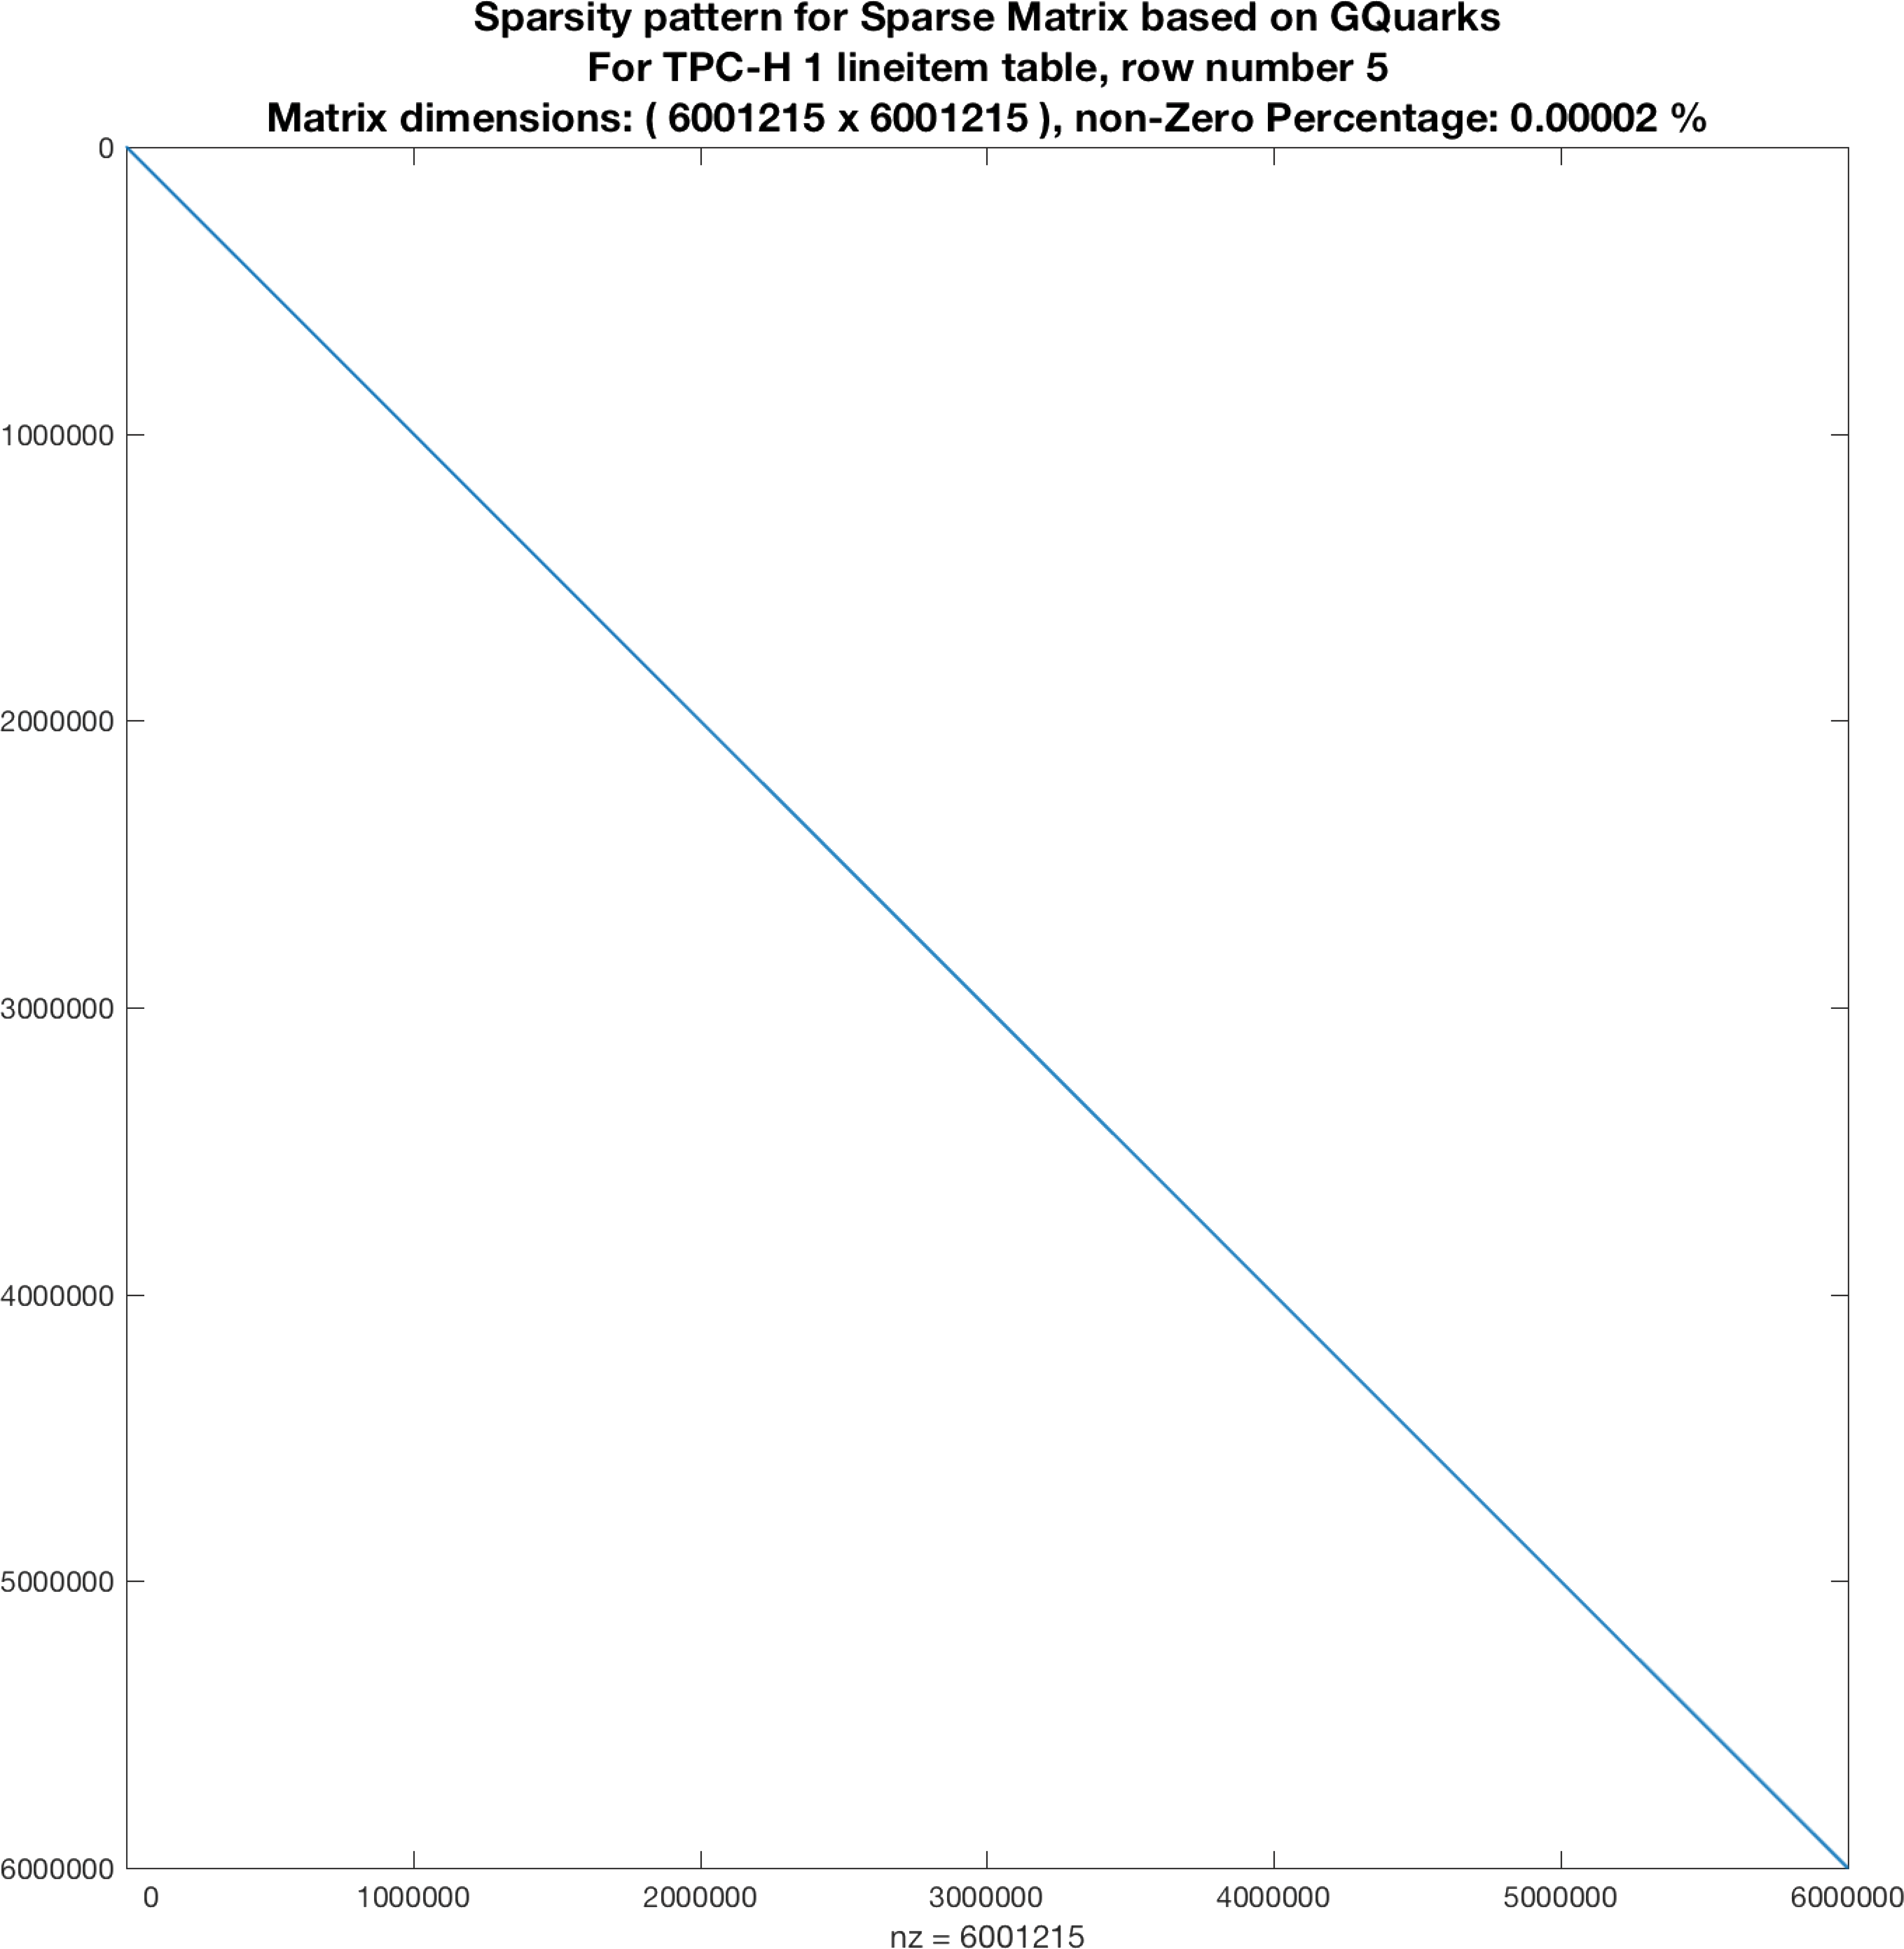
\includegraphics[width=1\columnwidth]{eps/sparsity_5.png}
\label{fig:sparse_1_5}
\end{figure}

\vspace{1.5cm}
\begin{figure}[H]
\centering
\caption{Sparsity pattern analysis for attribute return flag, from the TPC-H dataset 1GB lineitem table(column \#9).}
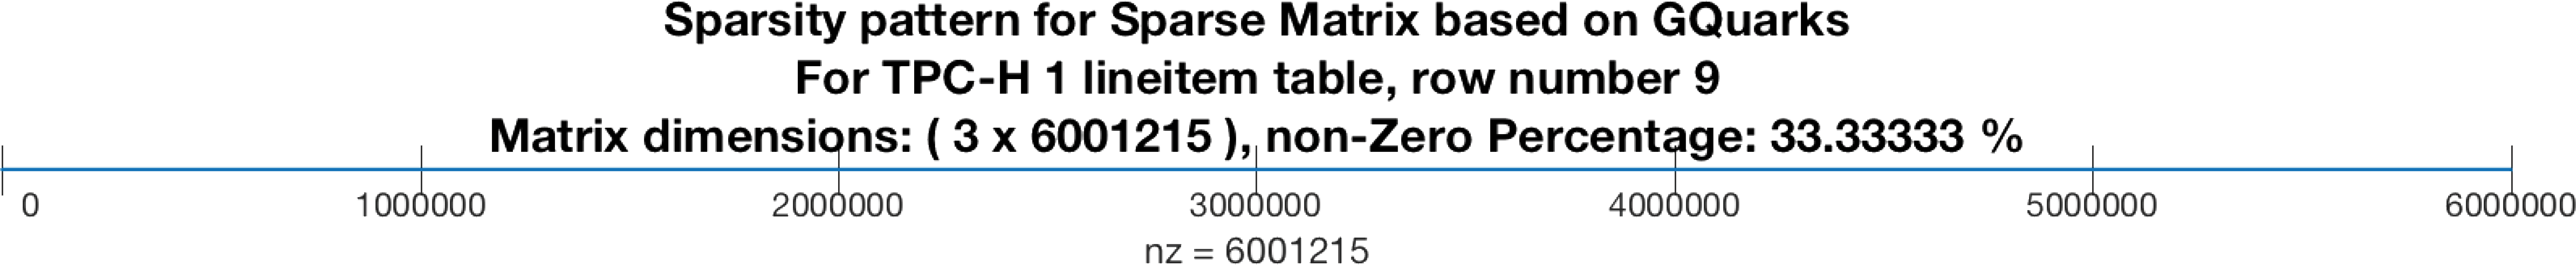
\includegraphics[width=1\columnwidth]{eps/sparsity_9.png}
\label{fig:sparse_1_9}
\end{figure}
\vspace{1.5cm}

\begin{figure}[H]
\centering
\caption{Sparsity pattern analysis for attribute line status, from the TPC-H dataset 1GB lineitem table(column \#10).}
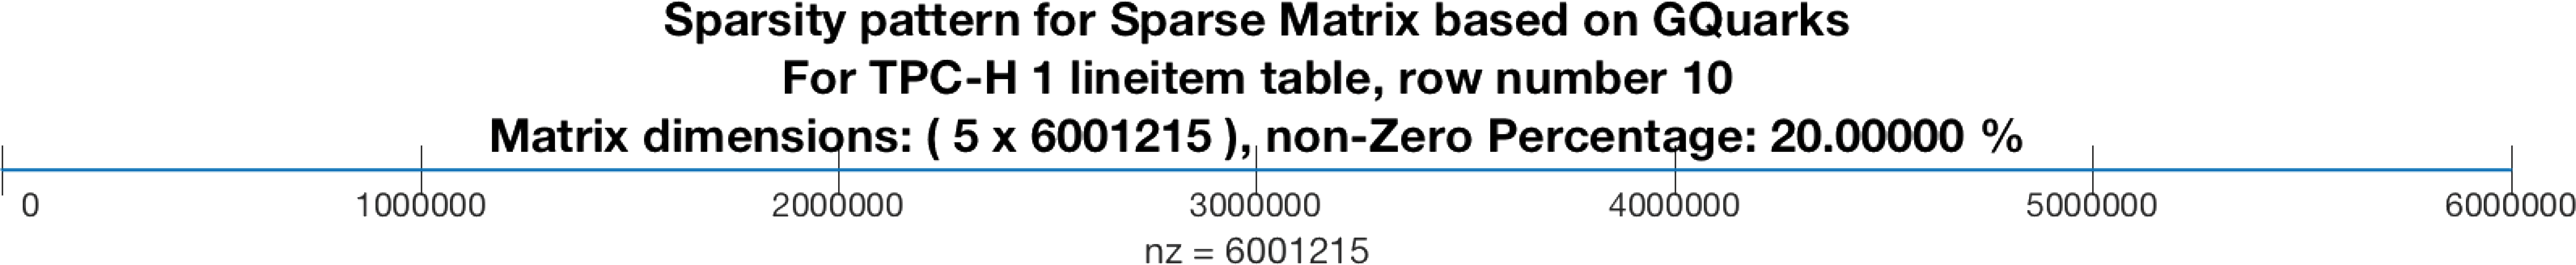
\includegraphics[width=1\columnwidth]{eps/sparsity_10.png}
\label{fig:sparse_1_10}
\end{figure}
\vspace{1.5cm}

\begin{figure}[H]
\centering
\caption{Sparsity pattern analysis for attribute shipdate, from the TPC-H dataset 1GB lineitem table(column \#11).}
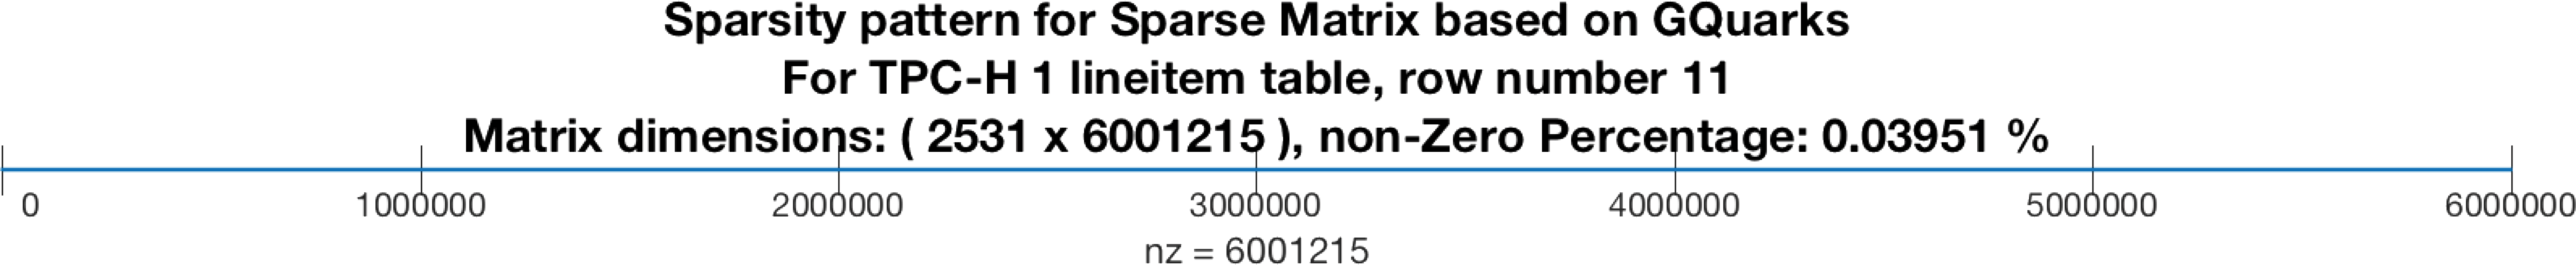
\includegraphics[width=1\columnwidth]{eps/sparsity_11.png}
\label{fig:sparse_1_11}
\end{figure}
\vspace{1.5cm}


As shown in the prior sparsity analysis, a matrix dimensions $(\ m\ \times\ n\ )$ will have, in the worst case, a non-zero number equal to n, since each column has at most one element. Therefore, to fully realise the potential of the processing units,  this memory bottleneck should be overcome.\par 
 Given the example matrix of figure \ref{fig:sparse_1_5}, the number of zero elements that would have to be stored and processed would be $(n-1)^2$. 
 
 Taking into account that for the 32GB TPC-H dataset  the number o element arises to 192,000,551, the necessary amount of memory to store only one single precision dense matrix would be  aproximately 150PB. \par 
 To explore data locality in cache memories to improve performance the design of the code should be consistent with the design of the caches. 
 The used matrices must also be compressed to take advantage of their mathematical structure. With the prior statements in mind the storage formats chosen  rely on the Compressed Sparse Column (CSC) and Compressed Sparse Row (CSR) formats \cite{silva2005sparse}. \par 
 Since each column has at most one element, the CSC format construction is thereby simplified, giving place to an sequential column pointer array, bigger in size in one element when compared to the value and row index arrays. Denote that after the LA selection operation the column pointer array no longer keeps the illustrated property. \par 
Regarding the usage of CSR format, it was chosen due to the creation of an alternative version to the LA operations that took CSC formatted matrices as input. This alternative version took CSR formatted matrices as input and relied on  Intel\textsuperscript{\textregistered} Math Kernel Library version 11.3.



\subsection{Incremental construction}
Projection matrices, as defined on section \ref{definition_matrices} are amenable to incremental construction due to the GQuarks lema, where each unique string will be associated to an unique unsigned integer. If the new data does not exist in terms of a GQuark, a new association will be created and a new unique unsigned integer will be associated to it. Regarding the consequent matrix column increase, due to register addition, no problem arises from that action.\par 
Dimension matrices, also defined on section \ref{definition_matrices}, only depend on the matrix column increase due to the direct association of the cell value, having also no problem regarding incremental construction.
Yesterday's data will still be valid and have zero migration cost with the addition of today's data.



    
 

